\clearpage\SourceLeaf{119}
\begin{center}\bfseries BEMERKUNGEN ZU DEN ELF\\PENTAGRAMM-FRAGMENTEN.\end{center}

Die zahlreichen Entwicklungen und Notizen über das »Pentagramma mirificum«, die sich in
\textsc{Gauss}' Nachlass gefunden haben, stammen aus sehr verschiedenen Zeiten und zeigen eine
vielfach wechselnde Bezeichnungsweise. Dem entsprechen die vielen verschiedenen
Standpunkte, von denen aus \textsc{Gauss} das Pentagramm betrachtete. Neben den acht in
Band III der Gesammelten Werke, S. 481 ff., veröffentlichten Fragmenten kommen in dieser Hinsicht noch
zwei Auffassungen in Betracht, die den drei oben abgedruckten Fragmenten
zugrunde liegen. Einige weitere unveröffentlichte Entwicklungen enthalten teils
Wiederholungen, teils ausführliche numerische Rechnungen zu dem von \textsc{Gauss} immer wieder
herangezogenen Beispiel mit $\alpha\beta\gamma\delta\varepsilon = 20$.

Um die Fragmente [9] bis [11] sachlich zu erläutern, muss man auf die
Fragmente [1] bis [8] zurückgreifen.

Als »Pentagramma mirificum« bezeichnet \textsc{Gauss} ein bereits von \textsc{Neper}\footnote{Da die
fraglichen Untersuchungen \textsc{Neper}s verhältnismäßig wenig bekannt sind, sei es erlaubt,
hier ein paar Bemerkungen darüber einzuschalten. Sie stehen in Liber II,
Caput IV
von \textsc{Neper}s »Mirifici Logarithmorum canonis descriptio« (Lugduni 1619) und
gipfeln in dem heute als »\textsc{Neper}sche Regel« bezeichneten Theorem. Sind $h$ die Hypotenuse,
$a, b$ die Katheten eines rechtwinkligen sphärischen Dreiecks und $\alpha, \beta$ die
den Seiten $a$ bzw. $b$ gegenüberliegenden Winkel, so sind mit $a, b, h, \alpha, \beta$ stets auch
\[
a' = \frac{\pi}{2}-h, \qquad b' = \frac{\pi}{2}-\beta, \qquad h' = \frac{\pi}{2}-b, \qquad
\alpha' = \frac{\pi}{2}-a, \qquad \beta' = \alpha
\]
fünf Bestimmungsstücke eines rechtwinkligen sphärischen Dreiecks gegeben. Der Übergang
vom ersten zum zweiten Dreieck ist dabei eine Operation, die sich nach fünfmaliger Wiederholung
von selbst schließt, da man dann zu den ursprünglichen Bestimmungsstücken
$a, b, h, \alpha, \beta$ zurückkehrt. \textsc{Neper} selbst sagt von dieser Regel, sie gehe
ganz unmittelbar aus der Figur eines Fünfecks hervor, wie es auch \textsc{Gauss} in den hier behandelten
Fragmenten untersucht. Geben wir tatsächlich in der gleich im Text näher
beschriebenen Figur dem auf der Kugel gedachten Dreieck $P_1P_2Q_4$ die Bestimmungsstücke
$\Arc{P_1Q_4}=a$, $\Arc{P_2Q_4}=b$, $\Arc{P_1P_2}=h$ usw., so erhält gerade das
benachbarte rechtwinklige Dreieck $P_2P_3Q_5$ die zuvor mit $a', b', h', \alpha',
\beta'$ bezeichneten Bestimmungsstücke. Man kann daher ein einzelnes
rechtwinkliges sphärisches Dreieck als Ausgangspunkt nehmen und von ihm aus durch
Verlängern zweier Seiten um ihre Komplemente und so weiter zu den übrigen vier Dreiecken der
Figur und damit zum Pentagramm gelangen. ---} bei seinen Untersuchungen über das rechtwinklige sphärische Dreieck benutztes sphärisches
Fünfeck ohne einspringende Winkel, in dem jede Ecke der Pol der Gegenseite
ist und die fünf Diagonalen daher Quadranten der Kugel sind. Alle diese
offenbar selbstpolaren Fünfecke bilden ein zweifach unendliches Kontinuum. Die
beigefügte Figur zeigt in stereografischer Projektion ein Pentagramm
$P_1P_2P_3P_4P_5$.

\begin{center}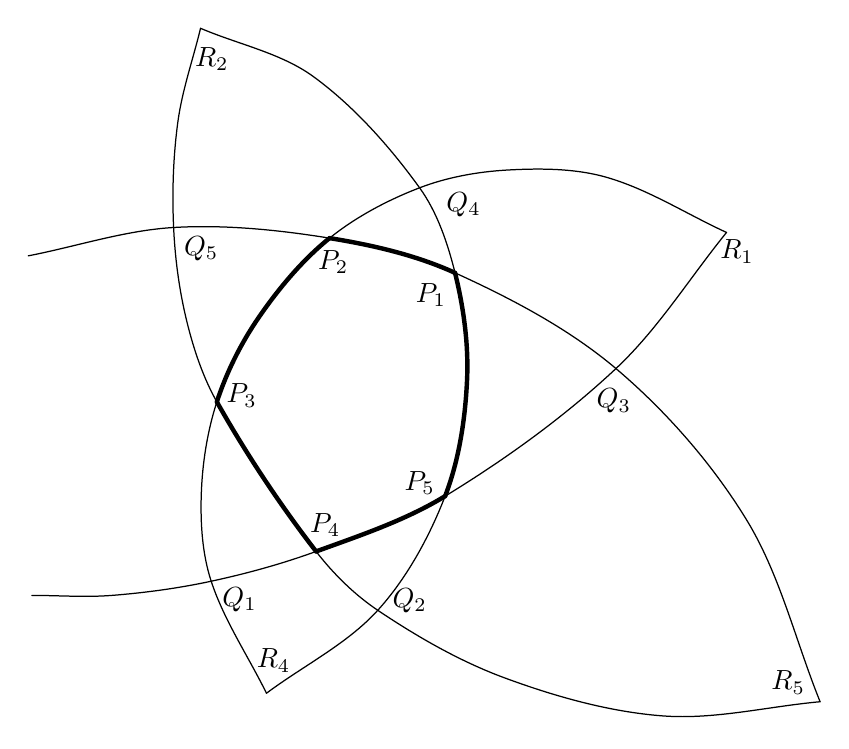
\begin{tikzpicture}[x=.009cm,y=-.009cm,line width=.45pt,line cap=round,line join=round,every node/.style={inner sep=0pt,font=\normalsize}]
\draw (30,336) .. controls (98.333,322.667) and (166.088,300.054) .. (235,296) .. controls (307.754,291.72) and (382.8,299.361) .. (455,311) .. controls (515.133,320.694) and (576.765,334.843) .. (632,360) .. controls (711.431,396.177) and (792.68,438.845) .. (859,495) .. controls (929.68,554.845) and (994.637,629.074) .. (1043,708) .. controls (1090.637,785.741) and (1112.333,879.333) .. (1147,965);
\draw[line width=1.6pt] (455,311) .. controls (515.133,320.694) and (576.765,334.843) .. (632,360);
\draw (35,815) .. controls (72.667,815) and (110.544,817.961) .. (148,815) .. controls (194.877,811.294) and (242.02,804.899) .. (288,795) .. controls (338.02,784.232) and (387.904,770.49) .. (436,753) .. controls (497.904,730.49) and (562.028,709.139) .. (618,675) .. controls (703.028,623.139) and (786.386,563.041) .. (859,495) .. controls (918.72,439.041) and (963,367) .. (1015,303);
\draw[line width=1.6pt] (436,753) .. controls (497.904,730.49) and (562.028,709.139) .. (618,675);
\draw (273,15) .. controls (262.333,59) and (247.038,102.352) .. (241,147) .. controls (234.371,196.019) and (232.728,246.548) .. (235,296) .. controls (237.062,340.882) and (243.206,386.471) .. (254,430) .. controls (263.54,468.471) and (276.537,507.458) .. (296,542) .. controls (337.203,615.124) and (384.695,686.552) .. (436,753) .. controls (460.362,784.552) and (490.015,813.844) .. (523,836) .. controls (578.348,873.177) and (638.442,907.813) .. (701,931) .. controls (772.442,957.48) and (849.434,979.239) .. (925,985) .. controls (998.101,990.573) and (1073,971.667) .. (1147,965);
\draw[line width=1.6pt] (296,542) .. controls (337.203,615.124) and (384.695,686.552) .. (436,753);
\draw (273,15) .. controls (326,37.667) and (386.337,49.75) .. (432,83) .. controls (489.337,124.75) and (540.299,182.245) .. (582,240) .. controls (606.966,274.578) and (621.666,318.357) .. (632,360) .. controls (644,408.357) and (651.209,460.287) .. (649,510) .. controls (646.543,565.287) and (637.872,623.584) .. (618,675) .. controls (595.872,732.251) and (564.027,790.74) .. (523,836) .. controls (480.027,883.406) and (418.333,914) .. (366,953);
\draw[line width=1.6pt] (632,360) .. controls (644,408.357) and (651.209,460.287) .. (649,510) .. controls (646.543,565.287) and (637.872,623.584) .. (618,675);
\draw (1015,303) .. controls (958.333,277) and (904.034,241.758) .. (845,225) .. controls (800.7,212.425) and (751.28,212.36) .. (705,215) .. controls (663.614,217.36) and (620.594,225.18) .. (582,240) .. controls (537.261,257.18) and (492.239,280.979) .. (455,311) .. controls (416.572,341.979) and (383.122,382.143) .. (355,423) .. controls (330.122,459.143) and (309.499,500.335) .. (296,542) .. controls (282.499,583.668) and (275.386,629.178) .. (274,673) .. controls (272.719,713.512) and (275.405,756.668) .. (288,795) .. controls (306.072,850.002) and (340,900.333) .. (366,953);
\draw[line width=1.6pt] (455,311) .. controls (416.572,341.979) and (383.122,382.143) .. (355,423) .. controls (330.122,459.143) and (309.499,500.335) .. (296,542);
\node at (289,58) {$R_2$};
\node at (1030,330) {$R_1$};
\node at (376,907) {$R_4$};
\node at (1102,938) {$R_5$};
\node at (274,326) {$Q_5$};
\node at (644,264) {$Q_4$};
\node at (856,541) {$Q_3$};
\node at (328,821) {$Q_1$};
\node at (568,823) {$Q_2$};
\node at (460,345) {$P_2$};
\node at (598,391) {$P_1$};
\node at (331,533) {$P_3$};
\node at (449,716) {$P_4$};
\node at (582,656) {$P_5$};
\end{tikzpicture}
\end{center}

Dieses wird von zwei weiteren, zwei- bzw. dreifach gewundenen Fünfecken begleitet,
$Q_1Q_3Q_5Q_2Q_4$ und $R_1R_4R_2R_5R_3$. Nach der Grundeigenschaft des Pentagramms sind
die Winkel dieser beiden Fünf\SourceLeaf{120}ecke durchweg rechte Winkel. Sind $s_k$ die Seitenlängen des Pentagramms $P_1\ldots P_5$ (bei
Kugelradius 1), so ergeben sich die Seiten der weiteren Fünfecke aus

\[
\Arc{P_kQ_{k+2}} = \frac{\pi}{2} - s_{k-2}, \qquad \Arc{P_kQ_{k-2}} = \frac{\pi}{2} - s_{k+2},
\]
\[
\Arc{Q_kR_{k+2}} = s_{k+1}, \qquad \Arc{Q_kR_{k-2}} = s_{k-1}.
\]

Unter den Pentagrammen befindet sich insbesondere ein reguläres. Es hat die Seitenlänge
$s = \operatorname{arc\,sin}\sqrt{\dfrac{-1+\sqrt{5}}{2}}$ und lässt sich aus dem sphärischen Dreieck mit den
Winkeln $\dfrac{2\pi}{5}, \dfrac{\pi}{2}, \dfrac{\pi}{4}$ durch Wiederholung um die Ecke des
ersten Winkels erzeugen.

Die soeben am allgemeinen Pentagramm aufgezeigten geometrischen Beziehungen lassen sich
mithilfe der Grundformeln des rechtwinkligen sphärischen Dreiecks als eine Reihe von
Gleichungen schreiben. Dies ist in den Fragmenten [1] und [3] ausgeführt. ---

Projiziert man das Pentagramm aus dem Kugelmittelpunkt auf eine Tangentialebene mit einem im
Pentagramm gelegenen Berührungspunkt $O$, so entsteht ein ebenes Fünfeck, in dem die fünf
Geraden $\overline{OP_k}$ die Höhen liefern. Das ebene Fünfeck hat somit die folgenden beiden
Eigenschaften, die es auch bestimmen.

1) Die fünf Höhen verlaufen alle durch denselben Punkt $O$.

2) Jede Höhe wird durch $O$ in zwei Stücke geteilt, deren Produkt für alle Höhen
gleich ist und dem Quadrat des Kugelradius entspricht.

\textsc{Gauss} verwendet nun die Projektionsebene zur Darstellung der komplexen Zahlen (vgl. Fragment [2])
und wählt insbesondere $O$ als Nullpunkt. Die weiteren Entwicklungen in Fragment [2]
haben folgenden Sinn. Auf fünf von $O$ ausgehenden Strahlen werden fünf
Punkte $p, p', \ldots, p''''$ beliebig gewählt. Die von \textsc{Gauss} angegebene Verschiebung
dieser Punkte auf ihren jeweiligen Strahlen bis in die Lagen $q, q', \ldots, q''''$ liefert
in den so erreichten Punkten die Ecken eines Pentagramms unserer Art. ---

Ist $M$ der Kugelmittelpunkt, so lässt sich durch die fünf zu den Pentagrammecken $P_k$
verlaufenden Strahlen $\overline{MP_k}$ ein eindeutig bestimmter Kegel zweiten Grades legen.
Dieser Kegel und insbesondere seine Trans\SourceLeaf{121}formation auf die Hauptachsen spielen in den weiteren Entwicklungen von \textsc{Gauss}
eine grundlegende Rolle. Die kubische Gleichung dieser Hauptachsentransformation, die
allein vom Produkt der fünf Tangenten der Pentagrammseiten abhängt, wird auch
numerisch in [5] behandelt. Will man die zahlreichen Beziehungen der
Fragmente [5] und [6] beweisen, so geht man am besten von den bekannten neueren
Grundformeln für die Hauptachsentransformation eines Kegels aus. In dem von \textsc{Gauss} zunächst
gewählten Koordinatensystem $x, y, z$ lassen sich aus diesen Grundformeln die Gleichungen
der genannten Fragmente fast ohne Rechnung ableiten. ---

Die Entwicklungen unter [7] und [8], die das Datum 1843 April 20 tragen, begründen die
Beziehung des Pentagramms zur Fünfteilung der elliptischen Funktionen.
Zweifellos hat \textsc{Gauss} diese Beziehung auf Anregung von \textsc{Jacobi}s Abhandlung Ȇber die
Anwendung der elliptischen Transcendenten auf ein bekanntes Problem der
Elementargeometrie«\footnote{\textsc{Crelle}s Journal, Bd. 3 (1828).} erkannt. \textsc{Jacobi} untersucht
dort Fünfecke, die jeweils einem Kreis eingeschrieben sind und zugleich einen zweiten Kreis
umschreiben, und zeigt ihre Beziehung zu den elliptischen Funktionen.

Um vom Pentagramm zum \textsc{Jacobi}schen Fünfeck überzugehen, projiziert man
das Pentagramm vom Kugelmittelpunkt auf diejenige Tangentialebene der Kugel, deren
Berührungspunkt der Schnittpunkt der Kugel mit der Kegelachse ist. Der Kegel wird von
dieser Projektionsebene in einer Ellipse geschnitten, der das projizierte Pentagramm
eingeschrieben ist. Die in der nebenstehenden Figur angedeutete affine Transformation liefert in
$P_1'P_2'\,..\,P_5'$ ein \textsc{Jacobi}sches Fünfeck.

\begin{center}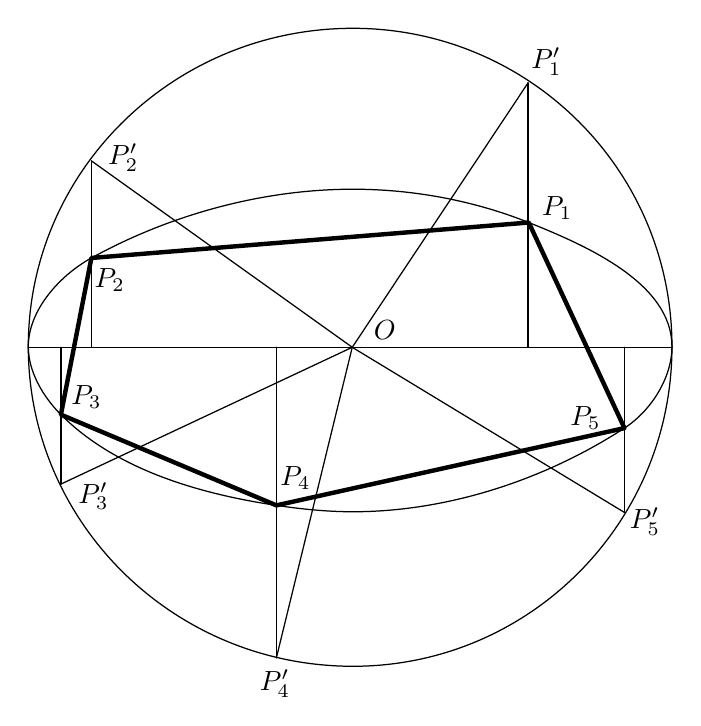
\begin{tikzpicture}[x=.009cm,y=-.009cm,line width=.45pt,line cap=round,line join=round,every node/.style={inner sep=0pt,font=\normalsize}]
\draw (41,480) .. controls (41,232) and (246,31) .. (499,31) .. controls (748,31) and (949,232) .. (949,480) .. controls (949,729) and (748,931) .. (499,931) .. controls (246,931) and (41,729) .. cycle;
\draw (41,480) .. controls (41,428.851) and (85.182,379.65) .. (130,355) .. controls (241.436,293.71) and (371.821,258) .. (499,258) .. controls (583.138,258) and (668.88,273.752) .. (747,305) .. controls (829.716,338.086) and (949,390.913) .. (949,480) .. controls (949,524.365) and (919.197,570.822) .. (882,595) .. controls (769.994,667.804) and (632.589,713) .. (499,713) .. controls (462.875,713) and (426.725,709.359) .. (391,704) .. controls (282.267,687.69) and (164.746,653.746) .. (87,576) .. controls (61.909,550.909) and (41,515.484) .. (41,480);
\draw (41,481)--(949,481);
\draw (498,481)--(746,108);
\draw (746,108)--(746,481);
\draw (498,481)--(130,218);
\draw (130,218)--(130,481);
\draw (498,481)--(87,674);
\draw (87,674)--(87,481);
\draw (498,481)--(391,919);
\draw (391,919)--(391,481);
\draw (498,481)--(882,714);
\draw (882,714)--(882,481);
\draw[line width=1.6pt] (747,305)--(130,355)--(87,576)--(391,704)--(882,595)--cycle;
\node at (772,78) {$P_1'$};
\node at (175,213) {$P_2'$};
\node at (133,691) {$P_3'$};
\node at (389,956) {$P_4'$};
\node at (911,727) {$P_5'$};
\node at (787,284) {$P_1$};
\node at (156,386) {$P_2$};
\node at (123,551) {$P_3$};
\node at (418,665) {$P_4$};
\node at (827,581) {$P_5$};
\node at (544,457) {$O$};
\end{tikzpicture}
\end{center}

Die Richtigkeit dieser Angaben zeigt sich an der Übereinstimmung der Formeln von \textsc{Gauss} in [7]
und [8] mit den von \textsc{Jacobi} an der zitierten Stelle entwickelten Gleichungen. Zum Beweis der
Beziehungen von \textsc{Gauss} kann man wie folgt vorgehen.

Benutzt man in der Projektionsebene die Hauptachsen der Ellipse als Achsen $x, y$ und setzt den
Kugelradius gleich 1, so liegt der Kugelmittelpunkt senkrecht zur Ebene unter $O$ in der
Entfernung 1. Die Grundeigenschaft des Pentagramms, dass nämlich
$\HistAngle P_{k-1}MP_{k+1} = \dfrac{\pi}{2}$ ist, liefert die fünf Gleichungen

\[
x_{k-1}x_{k+1} + y_{k-1}y_{k+1} + 1 = 0,\tag{1}
\]
\SourceLeaf{122}wobei $x_k, y_k$ die Koordinaten von $P_k$ sind. Jedes Paar $x_k, y_k$ kommt in zwei
Gleichungen vor, aus deren Auflösung man erhält

\[
x_k = \dfrac{y_{k+2}-y_{k-2}}{x_{k+2}y_{k-2}-x_{k-2}y_{k+2}}, \qquad
y_k = \dfrac{x_{k-2}-x_{k+2}}{x_{k+2}y_{k-2}-x_{k-2}y_{k+2}}.\tag{2}
\]

Ist nun, wie bei \textsc{Gauss}, $\varphi_k$ die exzentrische Anomalie von $P_k$, so sind die
Koordinaten von $P_k'$ offenbar $\cos\varphi_k, \sin\varphi_k$, und für die
Koordinaten von $P_k$ erhält man

\[
x_k = \sqrt{\dfrac{-G}{G'}}\cos\varphi_k, \qquad y_k = \sqrt{\dfrac{-G}{G''}}\sin\varphi_k,
\]

wobei $G, G'$ und $G''$ im Sinne von \textsc{Gauss} gebraucht sind. Setzt man diese Werte in die
Gleichungen (2) ein, so erhält man die ersten unter [7] angegebenen Gleichungen von \textsc{Gauss}.

\[
\dfrac{\cos\frac{1}{2}(\varphi_{k+2}+\varphi_{k-2})}{\cos\frac{1}{2}(\varphi_{k+2}-\varphi_{k-2})}
= \dfrac{G}{G'}\cos\varphi_k, \qquad
\dfrac{\sin\frac{1}{2}(\varphi_{k+2}+\varphi_{k-2})}{\cos\frac{1}{2}(\varphi_{k+2}-\varphi_{k-2})}
= \dfrac{G}{G''}\sin\varphi_k.
\]

Eliminiert man hier $\varphi_k$ und schreibt danach $k$ statt $k+2$, so folgt

\[
G'^2\cos^2\tfrac{1}{2}(\varphi_k+\varphi_{k+1}) + G''^2\sin^2\tfrac{1}{2}(\varphi_k+\varphi_{k+1})
= G^2\cos^2\tfrac{1}{2}(\varphi_k-\varphi_{k+1}),
\]
\[
G^2\cos(\varphi_{k+1}-\varphi_k) + (G''^2-G'^2)\cos\varphi_{k+1}+\varphi_k) = G'^2+G''^2-G^2.
\]

Durch Entwicklung der Kosinus und Einsetzen der Koordinaten der Punkte $P_k$ folgt weiter

\[
(G^2-G'^2+G''^2)G'x_kx_{k+1} + (G^2+G'^2-G''^2)G''y_ky_{k+1} +
(-G^2+G'^2+G''^2)G = 0.\tag{3}
\]

Nun sind $G, G', G''$ Wurzeln der Gleichung

\[
G(2G-1)^2 = \alpha\beta\gamma\delta\varepsilon(G-1).
\]

Für das Absolutglied der letzten Gleichung ergibt sich demnach

\[
(G^2+G'^2+G''^2-2G^2)G = \left(\dfrac{1+\alpha\beta\gamma\delta\varepsilon}{2} - 2G^2\right)G
= \dfrac{\alpha\beta\gamma\delta\varepsilon}{2}\cdot\dfrac{1}{2G-1},
\]

und man findet entsprechende Ausdrücke für die Koeffizienten der ersten beiden Glieder der
Gleichung (3), sodass sie übergeht in

\[
\dfrac{x_kx_{k+1}}{2G'-1} + \dfrac{y_ky_{k+1}}{2G''-1} + \dfrac{1}{2G-1} = 0.\tag{4}
\]

Behandelt man diese Gleichung ebenso wie (1), so ergeben sich die weiteren in Fragment
[7] zusammengestellten Beziehungen.

Die vorstehenden Angaben über die Beziehung zwischen \textsc{Gauss} und \textsc{Jacobi} erscheinen in einem neuen
Licht, wenn man bemerkt, dass jedes gewöhnliche Fünfeck ohne
einspringende Winkel durch eine Kollineation in ein \textsc{Jacobi}sches Fünfeck und damit auch in ein \textsc{Gauss}sches
Pentagramm transformiert werden kann. Dem gegebenen Fünfeck lässt sich nämlich eine
bestimmte Ellipse einschreiben und ein ebenso bestimmter Kegelschnitt umschreiben.
Man braucht dieses Kegelschnittpaar nur durch eine Kollineation in ein Kreispaar zu überführen,
was mit den heute bekannten Methoden keine Schwierigkeiten bereitet.

Diese Bemerkung ist auch für die Entwicklungen in den Fragmenten [9] bis [11]
wichtig. \textsc{Gauss} konstruiert hier zunächst durch wiederholtes Ziehen der Diagonalen bzw.
Verlängern der Seiten eine nach beiden
\SourceLeaf{123}Seiten hin unendliche Kette von Fünfecken und erkennt, dass dieses Netz einander umschließender Fünfecke

\begin{center}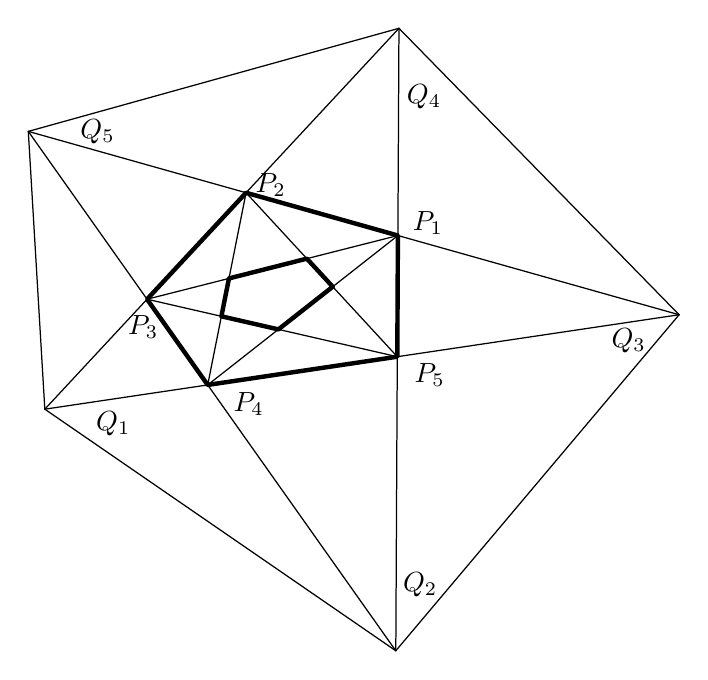
\begin{tikzpicture}[x=.01cm,y=-.01cm,line width=.45pt,line cap=round,line join=round,every node/.style={inner sep=0pt,font=\normalsize}]
\coordinate (Q5) at (392,534);
\coordinate (Q4) at (863,403);
\coordinate (Q3) at (1219,767);
\coordinate (Q2) at (859,1194);
\coordinate (Q1) at (413,887);
\coordinate (P2) at (668.717,611.962);
\coordinate (P1) at (861.668,666.325);
\coordinate (P5) at (860.89,820.317);
\coordinate (P4) at (619.971,856.186);
\coordinate (P3) at (542.909,747.276);
\draw (Q5)--(Q4);
\draw (Q4)--(Q3);
\draw (Q3)--(Q2);
\draw (Q2)--(Q1);
\draw (Q1)--(Q5);
\draw (Q5)--(Q3);
\draw (Q3)--(Q1);
\draw (Q1)--(Q4);
\draw (Q4)--(Q2);
\draw (Q2)--(Q5);
\draw (P2)--(P5);
\draw (P5)--(P3);
\draw (P3)--(P1);
\draw (P1)--(P4);
\draw (P4)--(P2);
\draw[line width=1.6pt] (P2)--(P1)--(P5)--(P4)--(P3)--cycle;
\draw[line width=1.6pt] (646.984,720.845)--(745.96,695.71)--(778.856,731.376)--(709.811,785.614)--(637.377,768.975)--cycle;
\node at (480,534) {$Q_5$};
\node at (895,490) {$Q_4$};
\node at (1155,800) {$Q_3$};
\node at (890,1110) {$Q_2$};
\node at (500,905) {$Q_1$};
\node at (700,602) {$P_2$};
\node at (900,650) {$P_1$};
\node at (902,844) {$P_5$};
\node at (672,880) {$P_4$};
\node at (538,783) {$P_3$};
\end{tikzpicture}
\end{center}

durch die Kollineation

\[
x' = \dfrac{2\,G-1}{2\,G'-1}\,x, \qquad y' = \dfrac{2\,G-1}{2\,G''-1}\,y\tag{5}
\]

in sich überführt wird. Zur Erläuterung dient die beigefügte Figur. \textsc{Gauss} hat selbst Zeichnungen dieser Art angefertigt, in denen die Fünfecknetze noch viel weiter fortgesetzt sind. Die auf der rechten Seite von (5) stehenden Koeffizienten sind die »Exponenten« oder »Coefficienten der Verjüngung«, die in [9] und [10] auftreten. Es liegt nahe, diesen Sachverhalt im Sinne der modernen Theorie der diskontinuierlichen Substitutionsgruppen aufzufassen. Der Nullpunkt $O$ erscheint dabei als der innere Grenzpunkt des Pentagrammnetzes und ist einer der drei Grenzpunkte der aus (5) hervorgehenden zyklischen Kollineationsgruppe.

Nach der vorangehenden Bemerkung liegt derselbe Sachverhalt bei jedem Fünfeck mit einspringenden Winkeln vor. Diese Verhältnisse sind in der neueren Literatur wohlbekannt.

Die Angaben von \textsc{Gauss} lassen sich folgendermaßen bestätigen. Das an $P_1P_2\,..\,P_5$ unmittelbar anschließende äußere Fünfeck $Q_1Q_2\,..\,Q_5$ ist dasselbe, das durch Projektion aus dem gleich bezeichneten sphärischen Fünfeck entsteht. Hat $Q_k$ die Koordinaten $x'_k$, $y'_k$, so gelten wegen $\HistAngle\,Q_kMP_{k+1} = \dfrac{\pi}{2}$ die fünf Gleichungen

\[
x'_k x_{k+1} + y'_k y_{k+1} + 1 = 0.
\]

Der Vergleich mit den fünf Gleichungen (4) lässt die Formeln (5) für alle Indizes $k$ als richtig erscheinen.

\SourceLeaf{124}
Dass \textsc{Gauss} den projektiven Charakter seiner zuletzt besprochenen Entwicklungen erkannt hat, macht insbesondere Fragment [11] wahrscheinlich. \textsc{Gauss} wendet hier die Grundsätze des baryzentrischen Kalküls von \textsc{Moebius} auf die Figur des geradlinigen Pentagramms an. Die Formeln von \textsc{Gauss} lassen sich im Sinne dieses Kalküls ohne Mühe verstehen. Dessen projektivem Charakter entsprechend geht man hier von einem beliebigen Fünfeck aus. Nach einem Brief an \textsc{Schumacher} vom 15. Mai 1843 hat \textsc{Gauss} erst am 14. Mai dieses Jahres das 1827 erschienene Werk von \textsc{Moebius} über den baryzentrischen Kalkül kennengelernt, vermutlich aus Anlass der Aufgabe, den Mittelpunkt eines durch fünf Punkte gegebenen Kegelschnitts durch Konstruktion zu finden. Für die speziellen Fünfecknetze, auf die sich die Formeln der Fragmente [5] bis [10] beziehen, wäre diese Aufgabe gleichbedeutend mit dem Problem, den inneren Grenzpunkt des einzelnen Netzes zu konstruieren. Die Entwicklungen der Fragmente [7] und [8] stammen aus dem April 1843, und die des Fragments [11] schließt sich wahrscheinlich unmittelbar an den 14. Mai 1843 an. Demnach darf man annehmen, dass die in [9] und [10] aufgenommenen Untersuchungen in den Wochen zwischen beiden Daten ausgeführt wurden.

\hfill\textsc{Fricke}.

\noindent\hrulefill\par
